\begin{homeworkProblem}
\begin{homeworkSection}{(a)}
To find the possible values of energy providing electron bound state  inside the MQW , the conbensional \textit{Transfer Matrix Method} is employed. Figure \ref{fig-MQW} shows eight castcaded quantume well which can be locally treated as a periodic structure. 
\begin{figure}[h]
\centering
% Generated with LaTeXDraw 2.0.8
% Mon Feb 18 08:10:56 GMT-06:00 2013
% \usepackage[usenames,dvipsnames]{pstricks}
% \usepackage{epsfig}
% \usepackage{pst-grad} % For gradients
% \usepackage{pst-plot} % For axes
\scalebox{0.4} % Change this value to rescale the drawing.
{
\begin{pspicture}(0,-1.4154687)(35.819965,1.4154687)
\psline[linewidth=0.04](17.800013,0.75953126)(18.526648,0.75953126)(18.526648,-1.1004688)(20.948729,-1.1004688)(20.948767,0.75953126)(21.675016,0.75953126)
\psline[linewidth=0.04](21.675016,0.75953126)(22.401651,0.75953126)(22.401651,-1.1004688)(24.823732,-1.1004688)(24.82377,0.75953126)(25.550018,0.75953126)
\psline[linewidth=0.04](25.550018,0.75953126)(26.276655,0.75953126)(26.276655,-1.1004688)(28.698736,-1.1004688)(28.698774,0.75953126)(29.425022,0.75953126)
\psline[linewidth=0.04](29.425022,0.75953126)(30.151657,0.75953126)(30.151657,-1.1004688)(32.57374,-1.1004688)(32.573776,0.75953126)(33.300026,0.75953126)
\psline[linewidth=0.04](2.3,0.75953126)(3.026636,0.75953126)(3.026636,-1.1004688)(5.4487166,-1.1004688)(5.448755,0.75953126)(6.175003,0.75953126)
\psline[linewidth=0.04](6.175003,0.75953126)(6.901639,0.75953126)(6.901639,-1.1004688)(9.32372,-1.1004688)(9.323758,0.75953126)(10.050006,0.75953126)
\psline[linewidth=0.04](10.050006,0.75953126)(10.776642,0.75953126)(10.776642,-1.1004688)(13.198723,-1.1004688)(13.198761,0.75953126)(13.92501,0.75953126)
\psline[linewidth=0.04](13.92501,0.75953126)(14.651646,0.75953126)(14.651646,-1.1004688)(17.073727,-1.1004688)(17.073765,0.75953126)(17.800013,0.75953126)
\psline[linewidth=0.04cm,arrowsize=0.12cm 2.2,arrowlength=1.5,arrowinset=0.4]{->}(33.54,0.31953126)(35.74,0.31953126)
\psline[linewidth=0.04cm,arrowsize=0.12cm 2.2,arrowlength=1.5,arrowinset=0.4]{->}(35.799965,-0.68932366)(33.600037,-0.6716139)
\usefont{T1}{ptm}{m}{n}
\rput(34.587345,0.7345312){\Large $A_N$}
\usefont{T1}{ptm}{m}{n}
\rput(34.607346,-1.0454688){\Large $D_N$}
\psline[linewidth=0.04cm,arrowsize=0.12cm 2.2,arrowlength=1.5,arrowinset=0.4]{->}(0.02,0.21953125)(2.22,0.21953125)
\psline[linewidth=0.04cm,arrowsize=0.12cm 2.2,arrowlength=1.5,arrowinset=0.4]{->}(2.2799644,-0.7893236)(0.08003564,-0.77161384)
\usefont{T1}{ptm}{m}{n}
\rput(1.0773437,0.63453126){\Large $A_0$}
\usefont{T1}{ptm}{m}{n}
\rput(1.0973438,-1.1454687){\Large $D_0$}
\usefont{T1}{ptm}{m}{n}
\rput(13.957344,1.1945312){\Large $L_b$}
\usefont{T1}{ptm}{m}{n}
\rput(15.857344,-0.72546875){\Large $L_w$}
\end{pspicture} 
}

\caption {MQW composed of eight castcaded quantum wells}
\label{fig-MQW}
\end{figure}

Suppose that the transfer matrix $\vp{M}_t$ relates $A_0$ and $D_0$ to $A_N$ and $D_N$ as:
\begin{equation}
\begin{bmatrix}
A_0\\
D_0
\end{bmatrix}
=
\begin{bmatrix}
M_{t}_{11} & M_{t}_{12}\\
M_{t}_{21}& M_{t}_{22}
\end{bmatrix}
\begin{bmatrix}
A_N\\
D_N
\end{bmatrix}
\end{equation}
To have bound states $A_0$ and $D_N$ should be zero ,that is, the outgoing part of the wavefunction outside of the MWQ should vanishes. This condition is translated as:
\begin{equation}\label{P3-1}
M_{t}_{11}=0
\end{equation}   
This equation is actually the characteristic equation which determines possible energies providing bound states inside the structure. To construct $\vp{M}_t$ we should first work on the transfer matrix assocoited with each unit cell. Figure \ref{fig-cell} shows a unite cell of the structure. The transfer matrix assocoited with this unite cell can be calculated by multiplying $\vp{M}_b(L_b/2)$ ,$\vp{M}_{bw}$, $\vp{M}_{w}(L_w)$ and $\vp{M}_{wb}$ as follows:
\begin{equation}
\vp{M}_{cell}=
\begin{bmatrix}\label{M_c}
m_{11} & m_{12}\\
m_{21} & m_{22}
\end{bmatrix}
=\vp{M}_{b}(L_b/2)\vp{M}_{bw}\vp{M}_{w}(L_w)\vp{M}_{wb}\vp{M}_{b}(L_b/2)
\end{equation}
\begin{figure}[h]
\centering
% Generated with LaTeXDraw 2.0.8
% Mon Feb 18 09:34:05 GMT-06:00 2013
% \usepackage[usenames,dvipsnames]{pstricks}
% \usepackage{epsfig}
% \usepackage{pst-grad} % For gradients
% \usepackage{pst-plot} % For axes
\scalebox{0.7} % Change this value to rescale the drawing.
{
\begin{pspicture}(0,-2.1854687)(15.494687,2.1854687)
\psline[linewidth=0.04](3.716875,1.3095312)(5.216875,1.3095312)(5.216875,-1.4904687)(10.216875,-1.4904687)(10.216875,1.3095312)(11.716875,1.3095312)
\usefont{T1}{ptm}{m}{n}
\rput(7.7342186,-0.85546875){\large $L_w$}
\usefont{T1}{ptm}{m}{n}
\rput(11.284219,1.9445312){\large $\frac{L_b}{2}$}
\usefont{T1}{ptm}{m}{n}
\rput(4.584219,1.9645313){\large $\frac{L_b}{2}$}
\usefont{T1}{ptm}{m}{n}
\rput(11.874219,-1.8954687){\large $\vp{M}_{b}\left(\frac{L_b}{2}\right)$}
\usefont{T1}{ptm}{m}{n}
\rput(3.5342188,-1.8954687){\large $\vp{M}_{b}\left(\frac{L_b}{2}\right)$}
\usefont{T1}{ptm}{m}{n}
\rput(10.054218,-1.9154687){\large $\vp{M}_{wb}$}
\usefont{T1}{ptm}{m}{n}
\rput(5.394219,-1.9154687){\large $\vp{M}_{bw}$}
\usefont{T1}{ptm}{m}{n}
\rput(7.784219,-1.9154687){\large $\vp{M}_w\left(L_{w}\right)$}
\end{pspicture} 
}

\caption{a unit cell of the MQW structure}
\label{fig-cell}
\end{figure}


where
\begin{equation}\label{P2-M_b}
\vp{M}_b(L_b/2)=
\begin{bmatrix}
\exp(k_bL_b/2) & 0\\
0 & \exp(k_bL_b/2)
\end{bmatrix}
\end{equation}

\begin{equation}
\vp{M}_{bw}=
\frac{1}{2}
\begin{bmatrix}
1-i\frac{k_w}{k_b}& 1+i\frac{k_w}{k_b}\\
 1+i\frac{k_w}{k_b} & 1-i\frac{k_w}{k_b}
\end{bmatrix}
\end{equation}

\begin{equation}
\vp{M}_w(L_w)=
\begin{bmatrix}
\exp(-ik_wL_w) & 0\\
0 & \exp(ik_wL_w)
\end{bmatrix}
\end{equation}

\begin{equation}\label{P2-M_wb}
\vp{M}_{wb}=
\frac{1}{2}
\begin{bmatrix}
1+i\frac{k_b}{k_w}& 1-i\frac{k_b}{k_w}\\
 1-i\frac{k_b}{k_w} & 1+i\frac{k_b}{k_w}
\end{bmatrix}
\end{equation}

In above equations $k_w$ and $k_b$ are the wavenumber in the wells and the barriers respectively:
\begin{align*}
k_w&=\sqrt{\frac{2m_{eff}E}{\hbar^2}}\\
k_b&=\sqrt{\frac{2m_{eff}(V_0-E)}{\hbar^2}}
\end{align*}
 By insering \eqref{P2-M_b}-\eqref{P2-M_wb} into \eqref{M_c} we obtain:
\begin{align}
&m_{11}=\exp(k_bL_b)\left[\cos(k_wL_w)-0.5\left(\frac{k_w}{k_b}-\frac{k_b}{k_w}\right)\sin(k_wL_w)\right]\\
&m_{12}=-0.5\exp(k_bL_b)\left(\frac{k_w}{k_b}+\frac{k2}{k1}\right)\sin(k_wL_w)\\
&m_{21}=0.5\exp(k_bL_b)\left(\frac{k_w}{k_b}+\frac{k2}{k1}\right)\sin(k_wL_w)\\
&m_{22}=\exp(-k_bL_b)\left[\cos(k_wL_w)+0.5\left(\frac{k_w}{k_b}-\frac{k_b}{k_w}\right)\sin(k_wL_w)\right]
\end{align}
 
Now we can calculate $\vp{M}_t$ by mmutiplying a series of transfer matrices of each unite cell:
\begin{equation}  
\vp{M}_t=\vp{M}_{cell}^{8}
\end{equation}

Based on the lecture the possible discrete energy eigenvalues for the bound state can be calculated by considering the possible continous energy bands for the infinite structure. In fact it is shown that the possible solutions satisfy the following condition:
\begin{equation}
U=\frac{1}{2}\left(m_{11}+m_{22}\right)\leq 1
\end{equation}
By evaluating $U$ as a function of $E$ allowable energy bands can be determined. Figure \ref{fig-P3-band} showes the continous energy bands for the infinite chain of wells.
\begin{figure}[h]
\centering
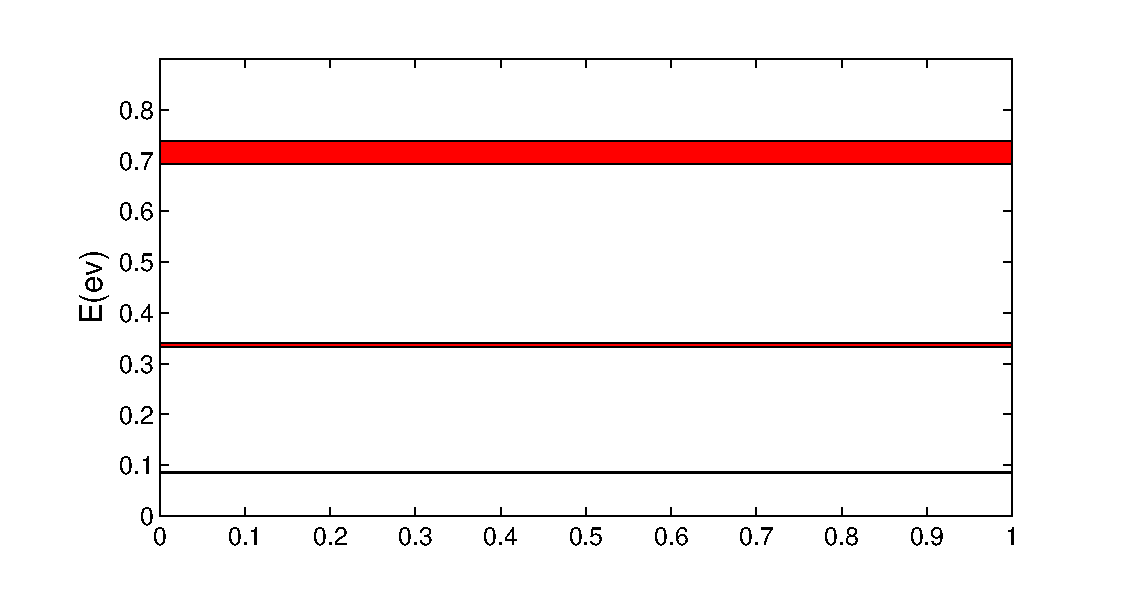
\includegraphics[scale=0.7]{energyband.eps}
\caption{continous energy bands for MQW}
\label{fig-P3-band}
\end{figure}
As explained previously to find discrete energy eigenfunctions for the bound sates we should find the solutions of \eqref{P3-1}. However $M_t_{11}$ flactuations are so striking and this makes our job diffcult. In fact  very fine meshes have to be used to find all zeros. To avoid comutational complexity we have used the notion of continous band structures:
\begin{enumerate}
\item
Find continous energy band using coarse meshes.(figure \ref{fig-P3-band})
\item
Search for the roots of $M_t_{11}$ inside each continous energy bands. It's expected that 8 zeros (solutions) can be fined inside each band. In this stage we should use more fine meshes.
\item
Refine your meshes near each approximate solution to get more precise solutions.
\end{enumerate} 
Figure \ref{fig-energysolutions} shows three $M_t_{11}$ inside three allowable energy bands. As it was expected in each region we have 8 solutions (correspond to eight QW).
\newpage
\begin{figure}[!h]
\begin{minipage}[b]{1\linewidth}
\centering
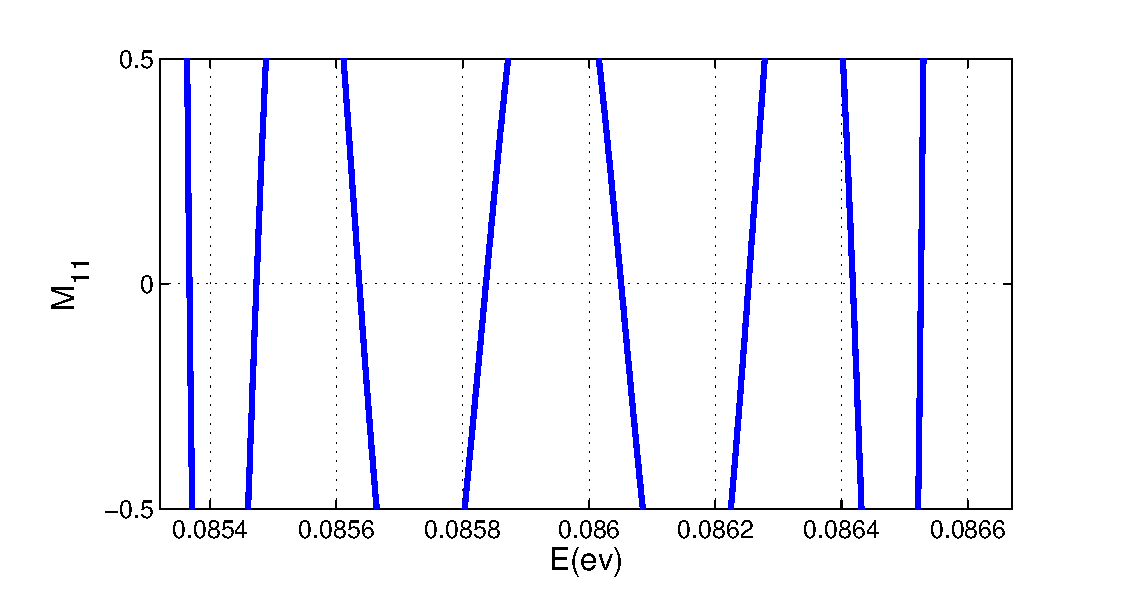
\includegraphics[scale=0.5]{M11_1.eps}
\centerline{\small (a) }
\end{minipage}
\begin{minipage}[b]{1\linewidth}
\centering
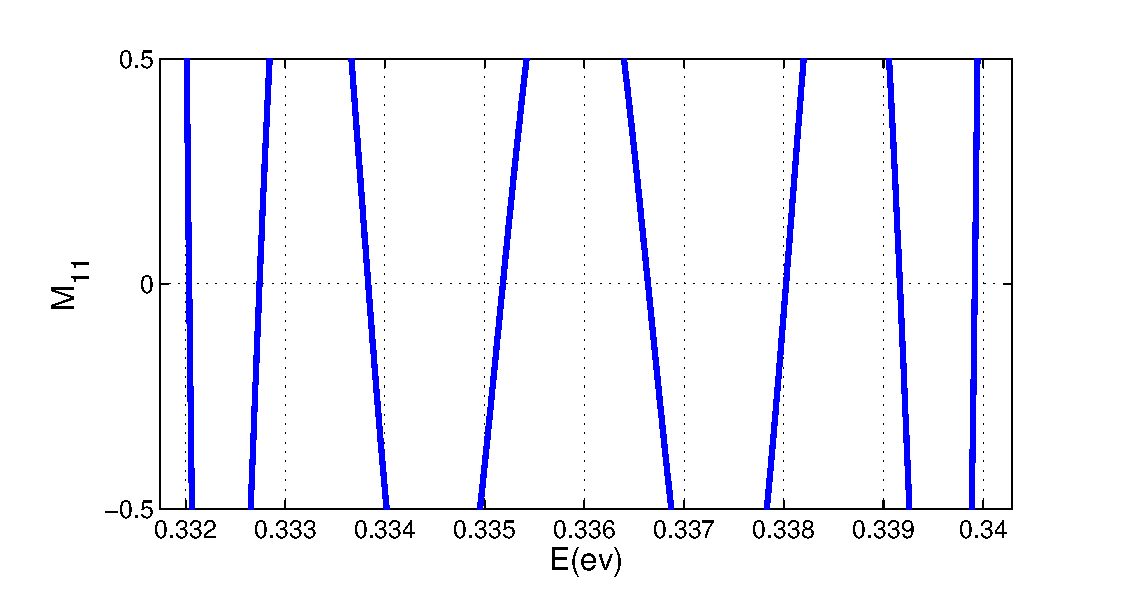
\includegraphics[scale=0.5]{M11_2.eps}
\centerline{\small (b) }
\end{minipage}
\begin{minipage}[b]{1\linewidth}
\centering
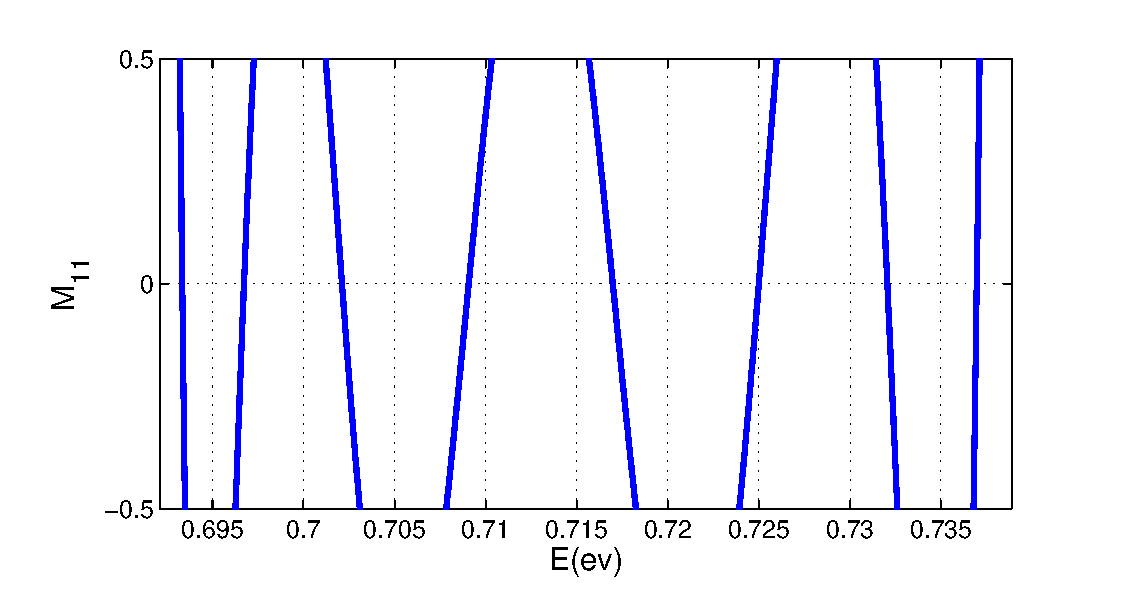
\includegraphics[scale=0.5]{M11_3.eps}
\centerline{\small (c) }
\end{minipage}
\caption { $M_t_{11}$ in three energy bands (a) fisrt band (b) second band and (c) third bad}
\label{fig-energysolutions}
\end{figure}
 Posible energy eigenvalues are given in table \ref{table}.
\begin{table}[!h]\centering
\caption{Energy eigenvalues for three bands (eV)}
\lr{\begin{tabular}{|c|c|c|c|c|c|c|c|c|}
\hline  8 &7 & 6 & 5 & 4 & 3 & 2 & 1 & n \\ \hline
\hline  0.0865 &   0.0864  &  0.0863  &  0.0861  &  0.0858  &  0.0856  &  0.0855  &  0.0854 & 1st band \\
\hline   0.3399  &  0.3392  &  0.3380  &  0.3366  &   0.3352  &  0.3338  &  0.3327  &  0.3320
 & 2nd band \\ 
 \hline   0.7370  &  0.7321  &  0.7250  &  0.7170  &  0.7091  &  0.7021  &  0.6967  &  0.6933 & 3rd band\\ 
\hline 
 \end{tabular}}
\label{table}
\end{table} 
 
\end{homeworkSection}

\begin{homeworkSection}{(b)}
As it's shown in figure \ref{fig-P3-band} there are two forbidden energy band inside first seventeen energy eigenvalues. Energy bands are shown in table \ref{table2}
 \begin{table}[!h]\centering
\caption{Energy bands (eV)}
\lr{\begin{tabular}{|c|c|}
\hline   0.0854-0.0866& 1st band \\
\hline  0.3318-0.3402 & 2nd band \\ 
 \hline   0.6922-0.7388 & 3rd band\\ 
\hline 
 \end{tabular}}
\label{table2}
\end{table} 

\end{homeworkSection}

\begin{homeworkSection}{(c)}
To find the wave function  for each energy eigenvalue we can utilize transfer matrices given in \eqref{P2-M_b}-\eqref{P2-M_wb}. Form the solution of the Schr\"odinger equation the wave function inside each region is:
\begin{align}
&\Psi^{b}_{n}(x)=A^{(b)}_{n}\exp\left[-k_b(x-b_n)\right]+D^{(b)}_n\exp\left[k_b(x-b_n)\right]\\
&\Psi^{w}_{n}(x)=A^{(w)}_{n}\exp\left[ik_w(x-w_n)\right]+D^{(w)}_n\exp\left[-ik_w(x-w_n)\right]
\end{align}
In above equations $\Psi^{b}_{n}(x)$ and $\Psi^{w}_{n}(x)$ are the wavefunction inside the nth barrier and nth well respectively. $b_n$ is the position of the center nth barrier and $w_n$ is the centrer of the nth well. to plot the wave function we follow the steps given below:
\begin{enumerate}
\item
select $A^{(b)}_1=1$ and $D^{(b)}_1=0$.
\item
use the transfer matrices to find $A_{n}^{(b)}$  and $D_{n}^{(b)}$  in term of $A_{n}^{(w)}$  and $D_{n}^{(w)}$ :
\begin{equation*}
\begin{bmatrix}
A_{n}^{(w)}\\
D_{n}^{(w)}
\end{bmatrix}
=\vp{M}_{w}(L_w/2)\vp{M}_{bw}\vp{M}_{b}(L_b/2)
\begin{bmatrix}
A_{n}^{(b)}\\
D_{n}^{(b)}
\end{bmatrix}
\end{equation*}
\item
evaluate $A_{n+1}^{(b)}$  and $D_{n+1}^{(b)}$:
\begin{equation*}
\begin{bmatrix}
A_{n+1}^{(b)}\\
D_{n+1}^{(b)}
\end{bmatrix}
=\vp{M}_{b}(L_b/2)\vp{M}_{bw}\vp{M}_{w}(L_w/2)
\begin{bmatrix}
A_{n}^{(b)}\\
D_{n}^{(b)}
\end{bmatrix}
\end{equation*}
\item
Normalize the wave function.
\end{enumerate} 

The wavefunctions for two energy eigenvalues are plotted in figures \ref{fig-psi_8} and \ref{fig-psi_9}. The computer program is given in the appendix.
\begin{figure}[!h]
\centering
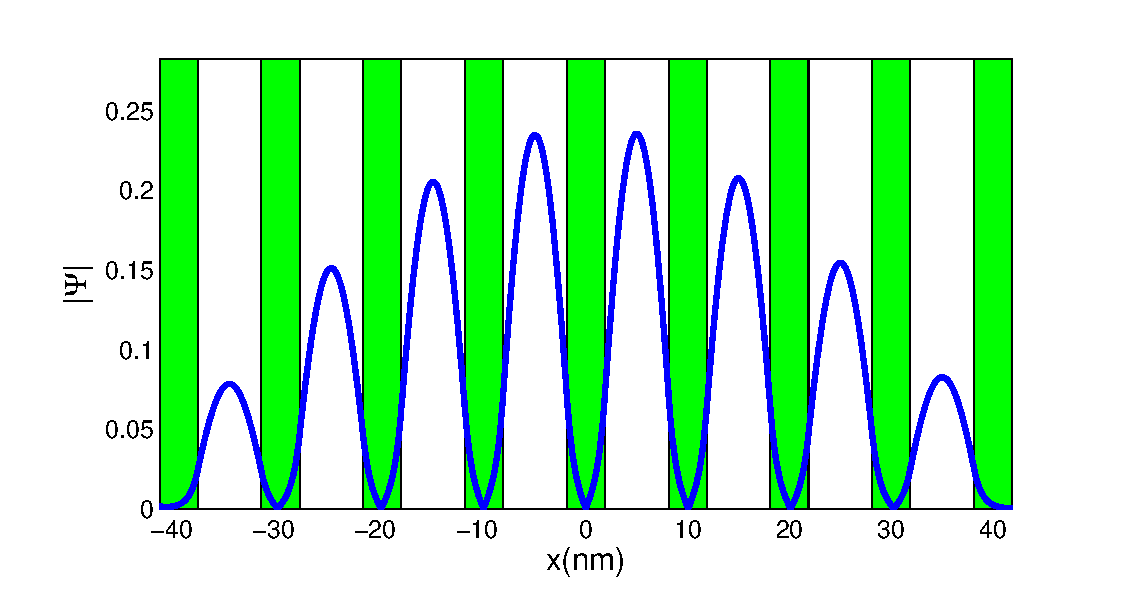
\includegraphics[scale=0.7]{psi_8.eps}
\caption{8th energy eigenfunction }
\label{fig-psi_8}
\end{figure}
\begin{figure}[!h]
\centering
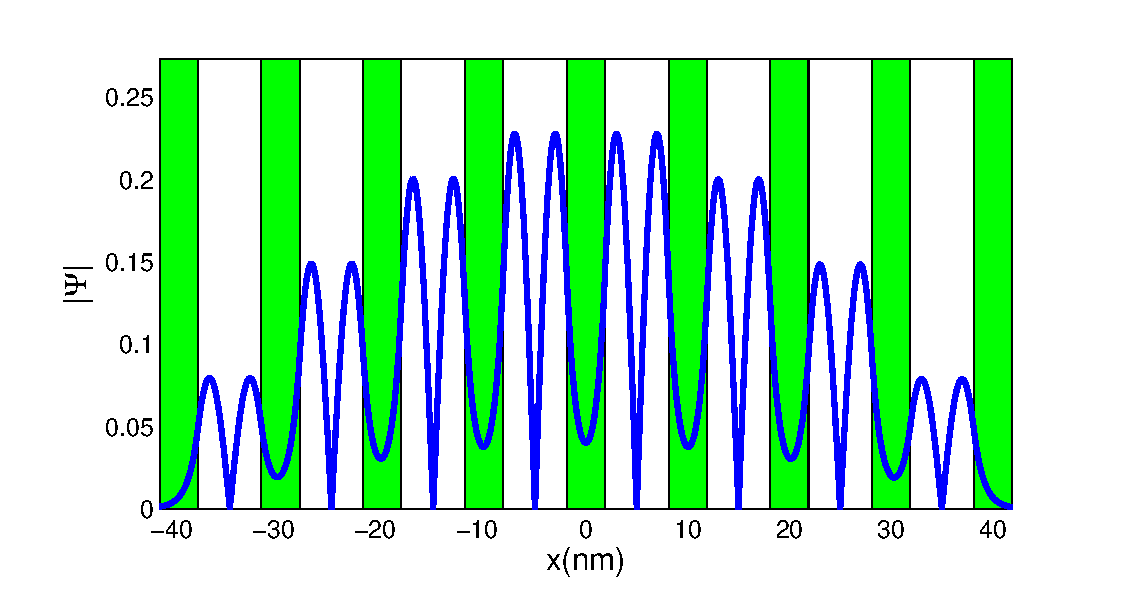
\includegraphics[scale=0.7]{psi_9.eps}
\caption{9th energy eigenfunction }
\label{fig-psi_9}
\end{figure}

\end{homeworkSection}


\end{homeworkPloblem}